\chapter{Release 1}
\section{Introduction}

Le terme release d\'{e}signe ici une version de notre application constitu\'{e}e d'une suite d'it\'{e}rations
qui se terminent quand les incr\'{e}ments de ces derniers construisent un produit pr\'{e}sentant
suffisamment de valeur \`{a} l'utilisateur.
Dans ce chapitre, nous allons nous int\'{e}resser \`{a} la premier release, de l'analyse des besoins
jusqu'au test. Nous traiterons en d\'{e}tails chacun des cas d'utilisation pr\'{e}alablement pr\'{e}sent\'{e}s.

\section{ Sprint 1 }


\subsection{Analyse}

    \textbf{ Diagramme de cas d'utilisation "G\'{e}rer un membre"}
    \begin{figure}[H]
    \center
    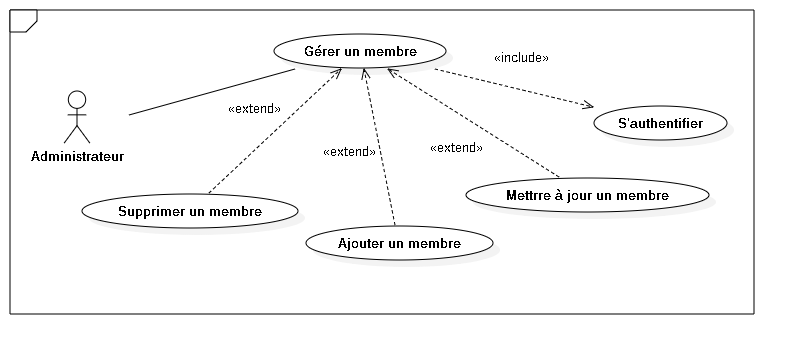
\includegraphics[width=13cm,height=8cm]{./figures/ucM.png}
    \caption{G\'{e}rer un membre.}

    \end{figure}

\subsection{Conception}

Le diagramme de s\'{e}quence indique l'interaction entre plusieurs acteurs
afin d'expliquer le d\'{e}roulement des diff\'{e}rents sc\'{e}nario entre les diff\'{e}rents
\'{e}l\'{e}ments du projet.

\subsubsection{Le sc\'{e}nario \guillemotleft{} Cr\'{e}ation d'un membre \guillemotright{}}

Le diagramme de s\'{e}quence \guillemotleft{} Ajout d'une t\^{a}che \guillemotright{} pr\'{e}sente le s\'{e}quencement
des interactions entre Administrateur, Application et Base de donn\'{e}es (BD).

\newpage
\subsection{Sch\'{e}ma}

\textbf{La table \guillemotleft{} members \guillemotright{}}

\begin{table}

\begin{tabular}{|l|l|l|l|l|l|}
\hline
Field        & Type         & Null & Key & Default            & Extra            \\
\hline
id           & int(11)      & NO   & PRI & NULL               & auto\_increment  \\
\hline
login        & varchar(30)  & YES  &     & NULL               &                  \\
\hline
password     & varchar(15)  & YES  &     & NULL               &                  \\
\hline
firstname    & varchar(50)  & YES  &     & NULL               &                  \\
\hline
lastname     & varchar(30)  & YES  &     & NULL               &                  \\
\hline
email        & varchar(100) & YES  &     & NULL               &                  \\
\hline
hiredate     & datetime     & YES  &     & CURRENT\_TIMESTAMP &                  \\
\hline
color        & varchar(6)   & YES  &     & NULL               &                  \\
\hline
projects\_id & int(11)      & YES  & MUL & NULL               &                  \\
\hline
pname        & varchar(50)  & YES  &     & NULL               &                  \\
\hline
\end{tabular}
\centering
 \caption {Members.}
\end{table}


\subsection{Test}

Dans ce premier sprint, nous testons la fonctionnalit\'{e}
« Gestion des membres» qui affiche, ajoute,
supprime les membres de la base de donn\'{e}es.
Ci-dessus nous ajoutons des captures \'{e}cran du sprint r\'{e}alis\'{e}.

\bigskip
\bigskip

Lors de la cr\'{e}ation d'un utilisateur , un email contenant son mot de passe lui
sera envoy\'{e}, ainsi si on modifie les param\'{e}tres d'utilisateur , un nouveeau
mot de passe lui sera envoy\'{e} sur la nouvelle addresse email .

\bigskip
\bigskip

\begin{figure}[H]
\center
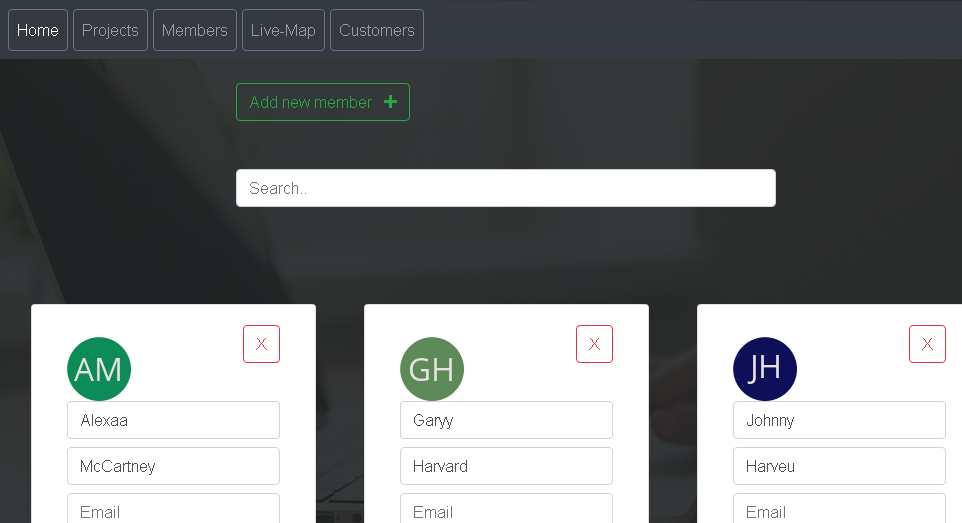
\includegraphics[width=11cm,height=7cm]{./figures/pres/mm1.png}
\caption{Gestion des membres.1.}
\end{figure}

\begin{figure}[H]
\center
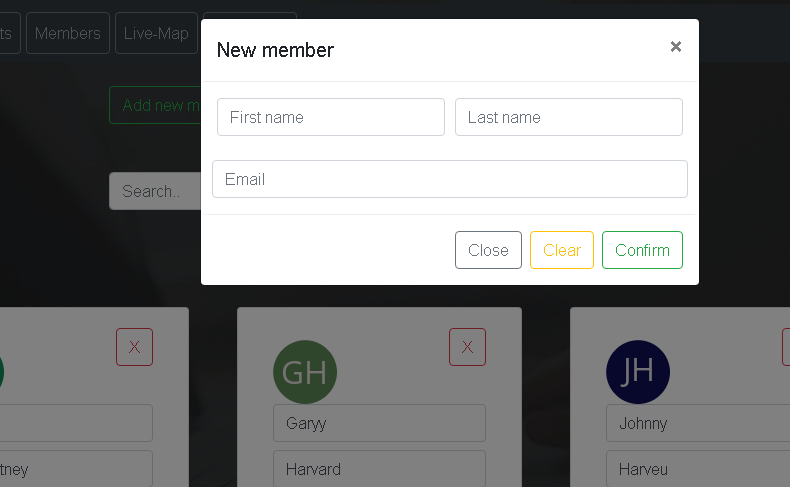
\includegraphics[width=11cm,height=7cm]{./figures/pres/mm2.png}
\caption{Gestion des membres.2.}
\end{figure}




\begin{figure}[H]
\center
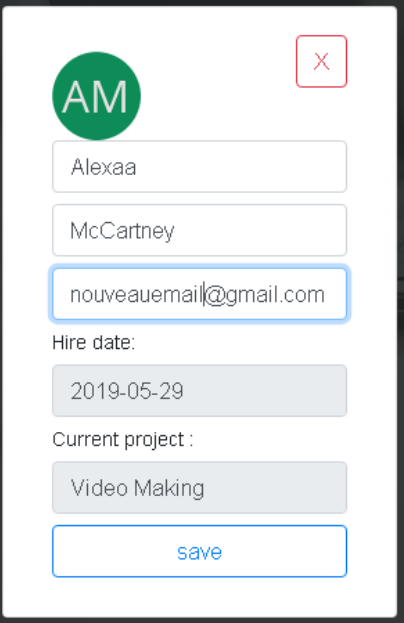
\includegraphics[width=11cm,height=7cm]{./figures/pres/mm3.png}
\caption{Gestion des membres.3.}
\end{figure}




\section{ Sprint 2 }
%clients

\subsection{Analyse}
\subsubsection{ Diagramme de cas d'utilisation "G\'{e}rer un client"}
\begin{figure}[H]
\center
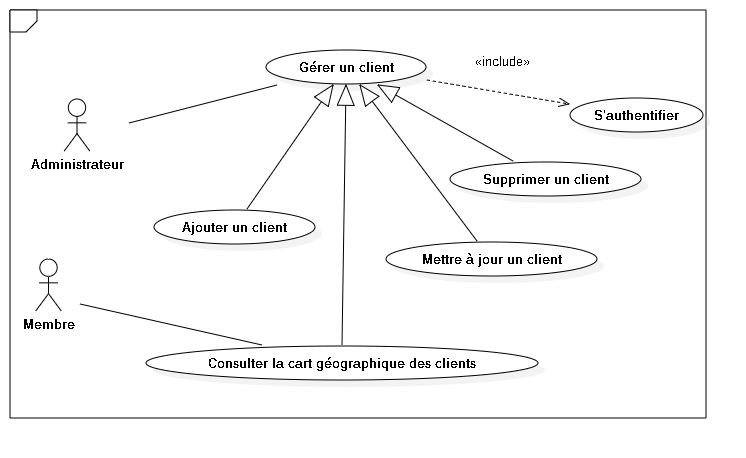
\includegraphics[width=13cm,height=8cm]{./figures/ucC.png}
\caption{G\'{e}rer un client.}
\end{figure}

\subsection{Conception}
\subsubsection{Le sc\'{e}nario \guillemotleft{} Cr\'{e}ation d'un client\guillemotright{}}
Le diagramme de s\'{e}quence \guillemotleft{} Ajout d'une t\^{a}che \guillemotright{} pr\'{e}sente le s\'{e}quencement
des interactions entre Administrateur, Application et Base de donn\'{e}es (BD).

\begin{figure}[H]
\center
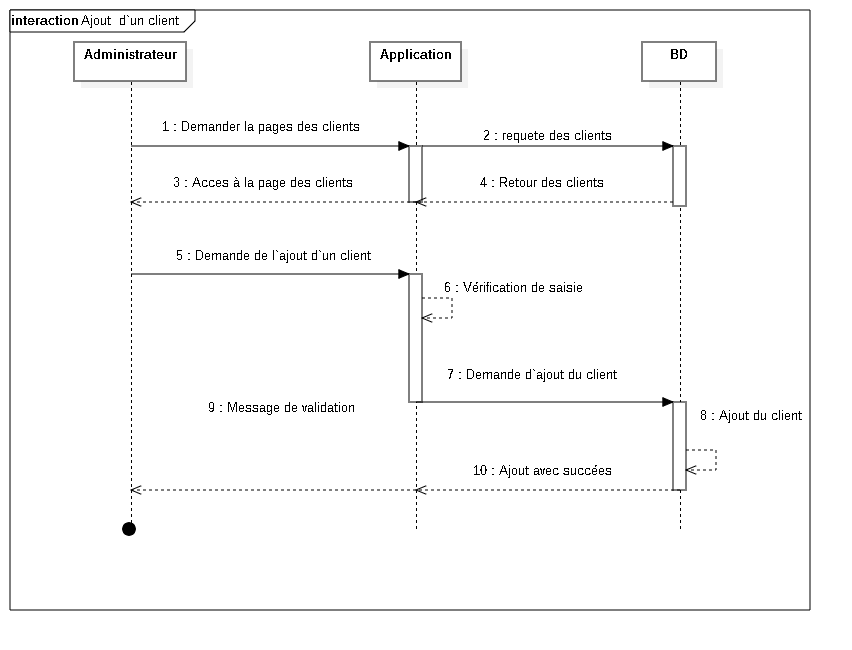
\includegraphics[width=14cm,height=9cm]{./figures/seq/F.png}
\caption{Cr\'{e}ation d'une client.}
\end{figure}



\subsubsection{Le sc\'{e}nario \guillemotleft{} Consultation de la carte g\'{e}ographique des clients\guillemotright{}}
Le diagramme de s\'{e}quence \guillemotleft{} Ajout d'une t\^{a}che \guillemotright{} pr\'{e}sente le s\'{e}quencement
des interactions entre Administrateur, Application et Base de donn\'{e}es (BD).



\subsubsection{Sch\'{e}ma}
\textbf{ La table \guillemotleft{} customers \guillemotright{}}


\begin{table}

\begin{tabular}{|l|l|l|l|l|l|}
\hline
Field            & Type          & Null & Key & Default            & Extra            \\
\hline
id               & int(11)       & NO   & PRI & NULL               & auto\_increment  \\
\hline
name             & varchar(45)   & YES  &     & NULL               &                  \\
\hline
phone            & varchar(45)   & YES  &     & NULL               &                  \\
\hline
address          & varchar(1000) & YES  &     & NULL               &                  \\
\hline
email            & varchar(50)   & YES  &     & NULL               &                  \\
\hline
longitude        & double        & YES  &     & NULL               &                  \\
\hline
latitude         & double        & YES  &     & NULL               &                  \\
\hline
subscriptionDate & datetime      & YES  &     & CURRENT\_TIMESTAMP &                  \\
\hline
\end{tabular}
\centering
\caption{Customers}
\end{table}


\subsection{Test}

\FloatBarrier
\begin{figure}[H]
\center
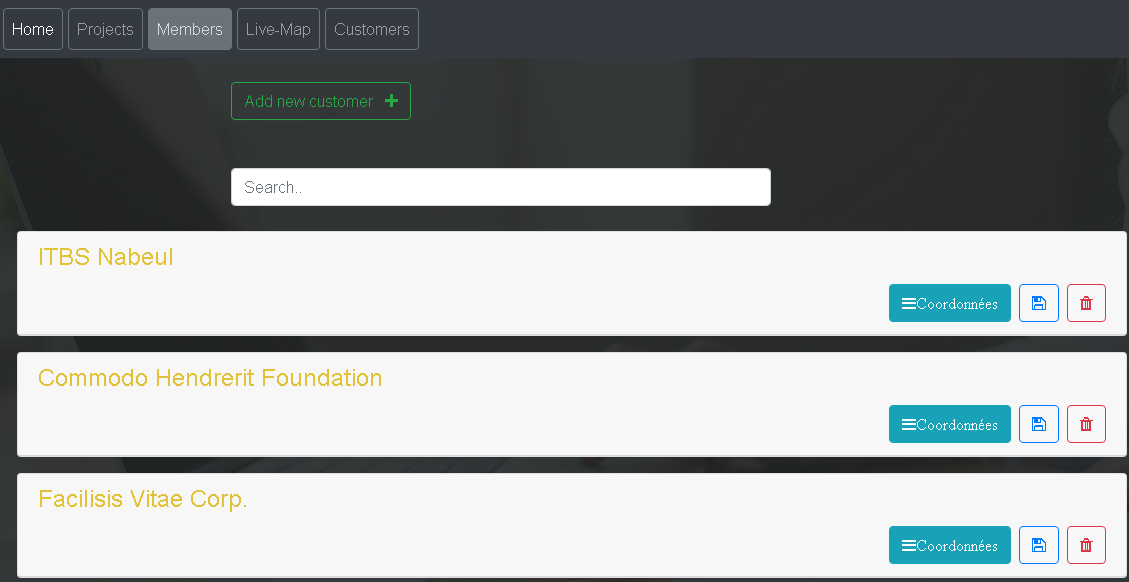
\includegraphics[width=11cm,height=7cm]{./figures/pres/cc1.png}
\caption{Gestion des clients.1.}
\end{figure}
\FloatBarrier


\FloatBarrier
\begin{figure}[H]
\center
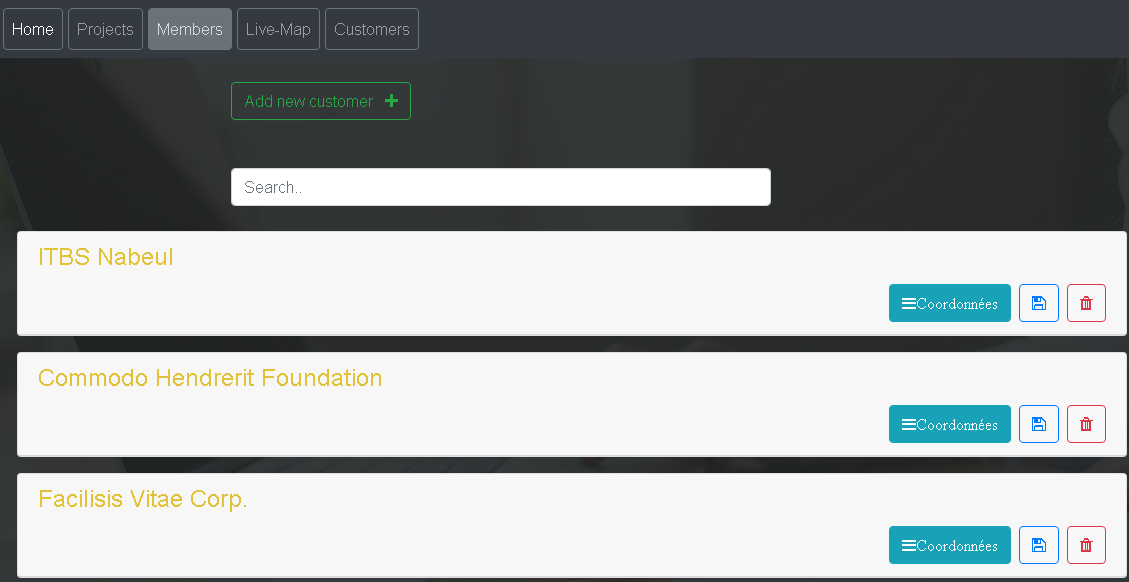
\includegraphics[width=11cm,height=7cm]{./figures/pres/cc1.png}
\caption{Gestion des clients.2.}
\end{figure}
\FloatBarrier
\subsection{Consultation carte g\'{e}ographique des clients}

\FloatBarrier
\begin{figure}[H]
\center
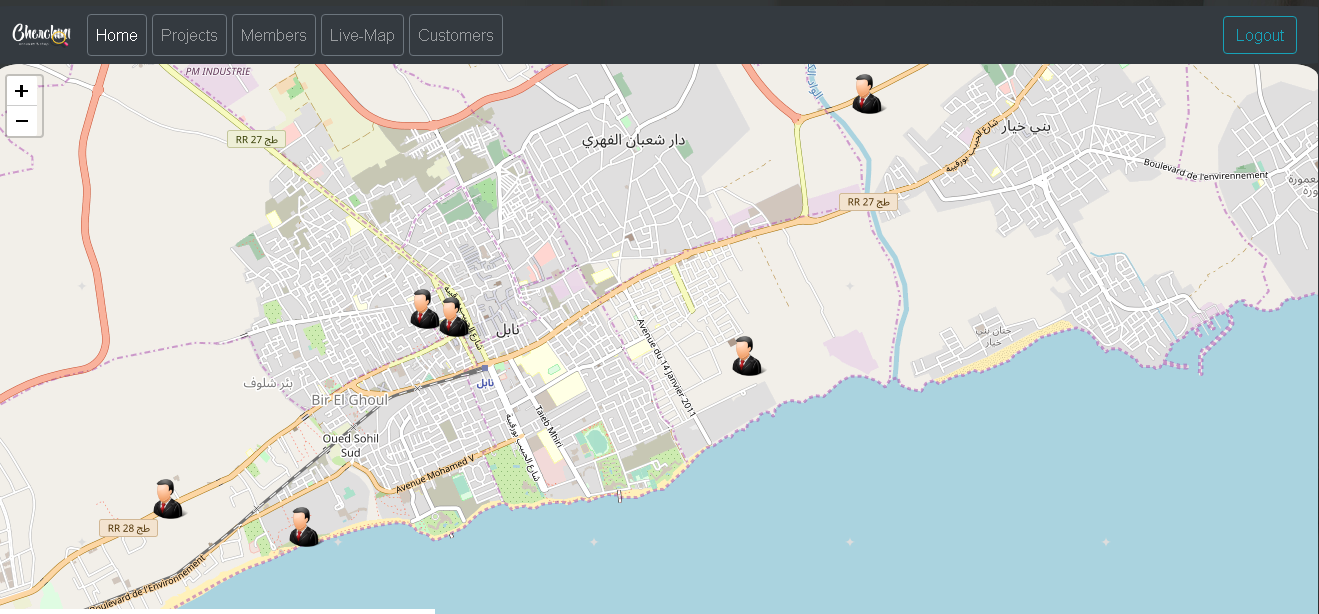
\includegraphics[width=15cm,height=10cm]{./figures/pres/map.png}
\caption{Carte g\'{e}ographique.}
\end{figure}
\FloatBarrier


\section{ Sprint 3 }
\subsubsection{Analyse}
\subsubsection{Conception}
\subsubsection{Code}
\subsubsection{Test}

\section{ Sprint 4 }
%auth

\subsection{Conception}
\textbf{Le sc\'{e}nario \guillemotleft{} Authentification \guillemotright{}}

Ce sch\'{e}ma pr\'{e}sente le m\^{e}me sc\'{e}nario pour l'administrateur et un simple
membre.(Figure 3.20) et (Figure 3.21)

\begin{figure}[H]
\center
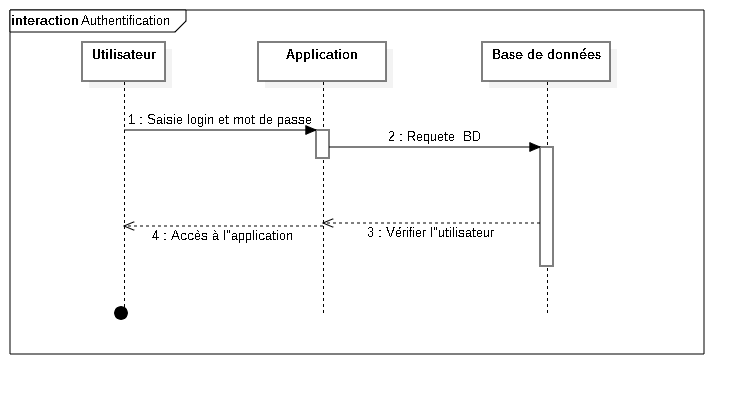
\includegraphics[width=14cm,height=8cm]{./figures/seq/A.png}
\caption{Authentification.}
\end{figure}


\subsection{Test}


\begin{figure}[H]
\center
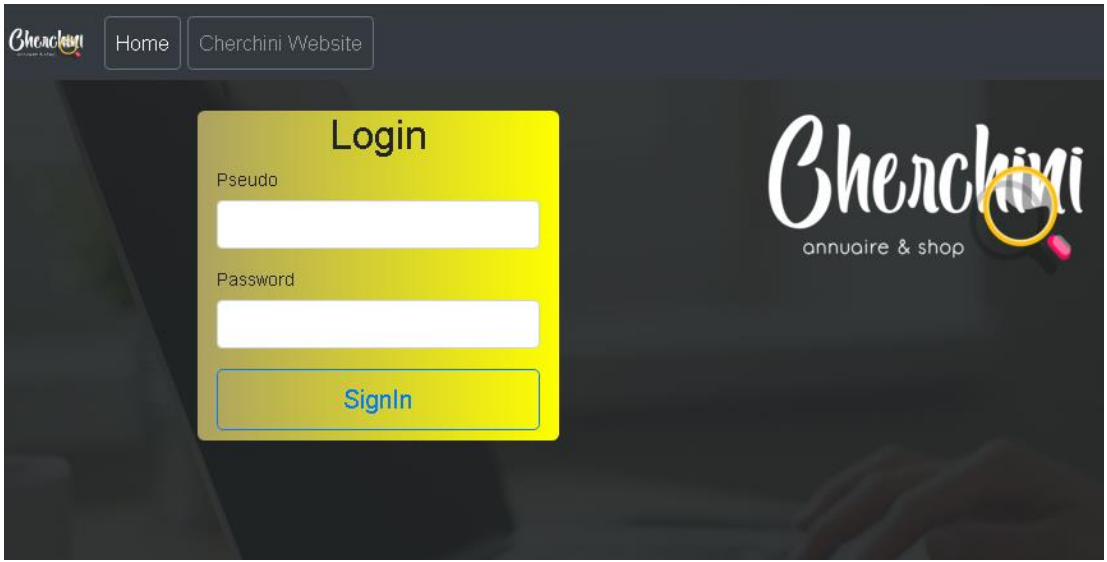
\includegraphics[width=11cm,height=7cm]{./figures/pres/1.png}
\caption{Accueil.}

\end{figure}


\section{ Sprint 5 }
%interface membre
\subsubsection{Analyse}

Le r\^{o}le  du membre consiste à modifier  l`\'{e}tat et la progression d'une t\^{a}che .
 \textbf{ Diagramme de cas d'utilisation "G\'{e}rer une t\^{a}che "}
    \begin{figure}[H]
    \center
    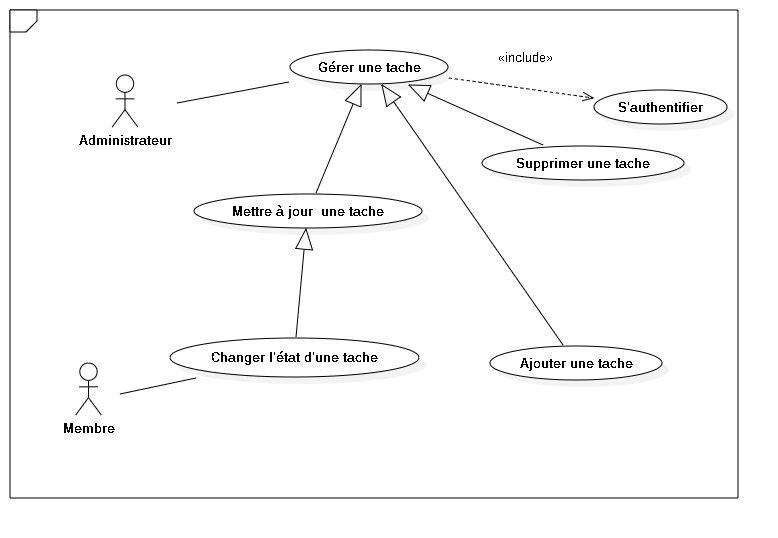
\includegraphics[width=13cm,height=8cm]{./figures/ucT.png}
    \caption{G\'{e}rer une  t\^{a}che.}

    \end{figure}

\subsubsection{Conception}
\textbf{ Le sc\'{e}nario \guillemotleft{} Modification de l`\'{e}tat d'une t\^{a}che\guillemotright{}}

Le diagramme de s\'{e}quence \guillemotleft{} Ajout d'une t\^{a}che \guillemotright{} pr\'{e}sente le s\'{e}quencement
des interactions entre Administrateur, Application et Base de donn\'{e}es (BD).


\begin{figure}[H]
\center
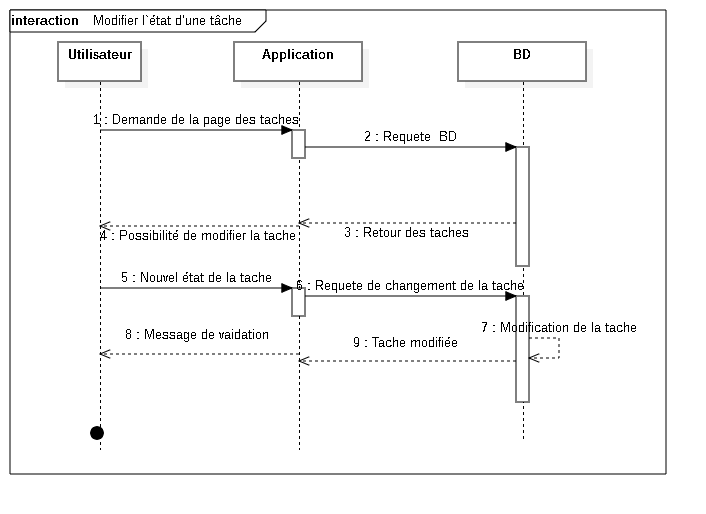
\includegraphics[width=14cm,height=10cm]{./figures/seq/D.png}
\caption{ Modification de l`\'{e}tat d'une t\^{a}che.}
\end{figure}

\begin{figure}[H]
\center
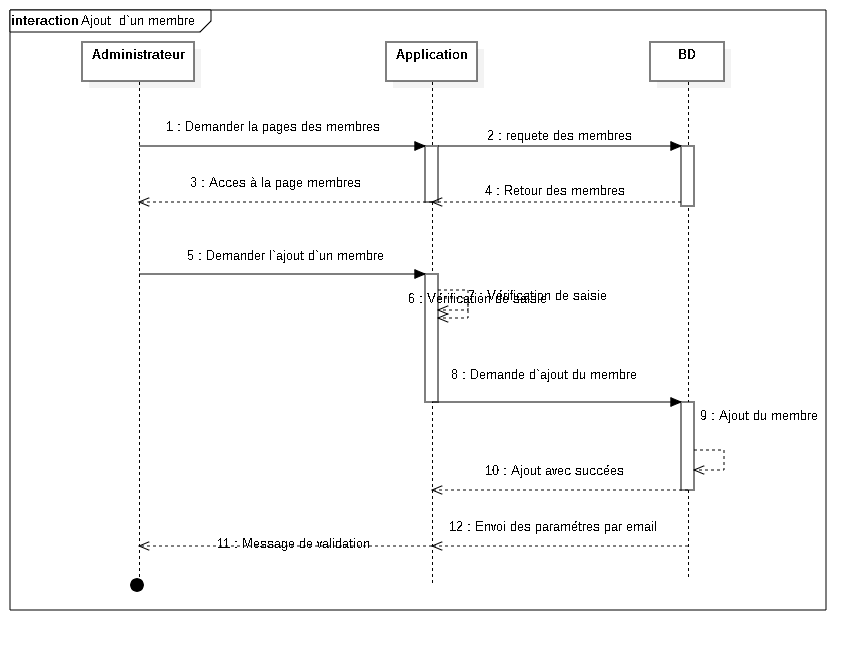
\includegraphics[width=14cm,height=10cm]{./figures/seq/E.png}
\caption{Cr\'{e}ation d'un membre.}
\end{figure}

\subsubsection{Sch\'{e}ma}
\begin{table}

\begin{tabular}{|l|l|l|l|l|l|}
\hline
Field        & Type         & Null & Key & Default            & Extra            \\
\hline
id           & int(11)      & NO   & PRI & NULL               & auto\_increment  \\
\hline
login        & varchar(30)  & YES  &     & NULL               &                  \\
\hline
password     & varchar(15)  & YES  &     & NULL               &                  \\
\hline
firstname    & varchar(50)  & YES  &     & NULL               &                  \\
\hline
lastname     & varchar(30)  & YES  &     & NULL               &                  \\
\hline
email        & varchar(100) & YES  &     & NULL               &                  \\
\hline
hiredate     & datetime     & YES  &     & CURRENT\_TIMESTAMP &                  \\
\hline
color        & varchar(6)   & YES  &     & NULL               &                  \\
\hline
projects\_id & int(11)      & YES  & MUL & NULL               &                  \\
\hline
pname        & varchar(50)  & YES  &     & NULL               &                  \\
\hline
\end{tabular}
\centering
\caption{Tasks}
\end{table}

\subsubsection{Test}

Si un simple membre est authentifi\'{e} par son mot de passe il sera amen\'{e}e \`{a}
l'interface \guillemotleft{} gestion de taches \guillemotright{} dans laquelle il peut modifier l'\'{e}tat des
taches .(ToDo ,Doing,Done ) et La progression des taches .


\begin{figure}[H]
\center
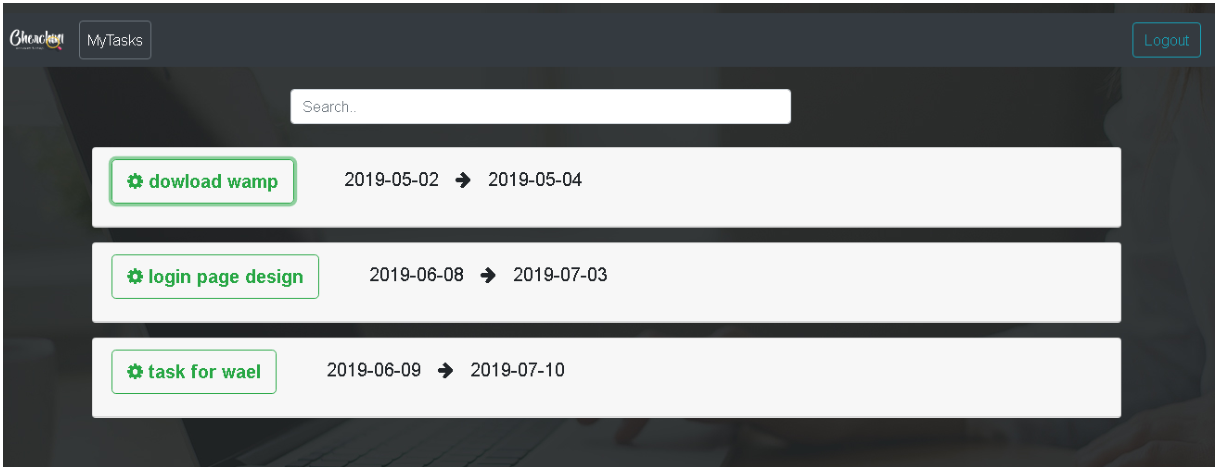
\includegraphics[width=11cm,height=7cm]{./figures/pres/2.png}
\caption{Espace membre.1.}

\end{figure}



\begin{figure}[H]
\center
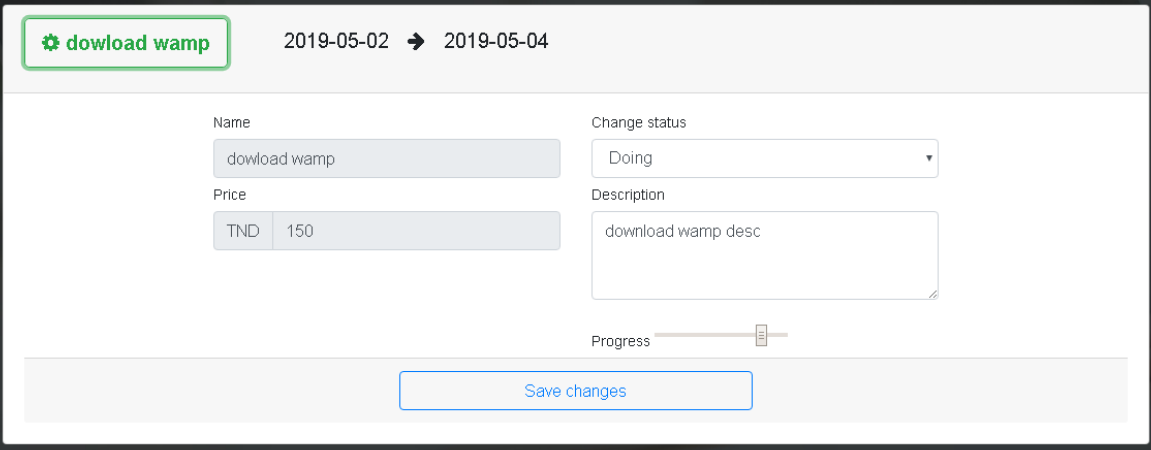
\includegraphics[width=11cm,height=7cm]{./figures/pres/3.png}
\caption{Espace membre.2.}

\end{figure}
 

\section{ Sprint 6 }
\input{sp16.tex}
